\documentclass[tikz]{standalone}
\usetikzlibrary{arrows,shapes,automata,petri,positioning}



\begin{document}
	
	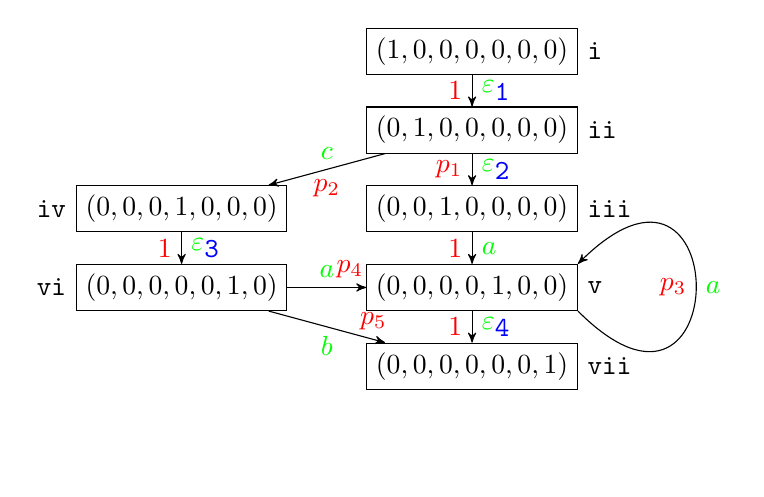
\begin{tikzpicture}[node distance=0.4cm and 1cm,>=stealth',bend angle=45,auto]
	
	
\node[draw=black,rectangle,label=right:{\texttt{i}}] (i) {$(1,0,0,0,0,0,0)$};
\node[draw=black,rectangle,label=right:{\texttt{ii}}] (ii) [below=of i] {$(0,1,0,0,0,0,0)$};


\node[draw=black,rectangle,label=right:{\texttt{iii}}] (iii) [below=of ii] {$(0,0,1,0,0,0,0)$};
\node[draw=black,rectangle,label=left:{\texttt{iv}}] (iv) [below left=of ii] {$(0,0,0,1,0,0,0)$};

\node[draw=black,rectangle,label=right:{\texttt{v}}] (v) [below=of iii] {$(0,0,0,0,1,0,0)$};
\node[draw=black,rectangle,label=left:{\texttt{vi}}] (vi) [below=of iv] {$(0,0,0,0,0,1,0)$};
\node[draw=black,rectangle,label=right:{\texttt{vii}}] (vii) [below=of v] {$(0,0,0,0,0,0,1)$};

\draw[->] (i) -- (ii) node [midway,right] {$\color{green}\varepsilon_\texttt{\color{blue}1}$} node [midway,left] {$\color{red}1$};
\draw[->] (ii) -- (iii) node [midway,right] {$\color{green}\varepsilon_\texttt{\color{blue}2}$} node [midway,left] {$\color{red}p_1$};
\draw[->] (ii) -- (iv) node [midway,above] {$\color{green}c$} node [midway,below] {$\color{red}p_2$};
\draw[->] (v.south east) .. controls +(2,-2) and +(2,2) .. (v.north east) node [midway,right] {$\color{green}a$} node [midway,left] {$\color{red}p_3$};
\draw[->] (vi) -- (v) node [midway] {$\color{green}a$} node [midway,above right] {$\color{red}p_4$};
\draw[->] (iii) -- (v) node [midway] {$\color{green}a$} node [midway,left] {$\color{red}1$};
\draw[->] (iv) -- (vi) node [midway] {$\color{green}\varepsilon_\texttt{\color{blue}3}$} node [midway,left] {$\color{red}1$};
\draw[->] (vi) -- (vii) node [midway,below] {$\color{green}b$} node [pos=0.9,above] {$\color{red}p_5$};
\draw[->] (v) -- (vii) node [midway] {$\color{green}\varepsilon_\texttt{\color{blue}4}$} node [midway,left] {$\color{red}1$};
	
%\node[draw=black,rectangle,label=right:{\texttt{\color{blue}i}}] (a) {$(1,0,0,0,0,0,0)$};
%\node[draw=black,rectangle,label=right:{\texttt{\color{blue}ii}}] (b) [below= of a] {$(0,1,0,0,1)$};
%\node[draw=black,rectangle,label=right:{\texttt{\color{blue}iii}}] (c) [below left= of b] {$(0,0,1,0,1)$};
%\node[draw=black,rectangle,label=right:{\texttt{\color{blue}iv}}] (d) [below right= of b] {$(0,1,0,0,0,1,0,0,0)$};
%\node[draw=black,rectangle,label=right:{\texttt{\color{blue}v}}] (g) [below = of d] {$(0,0,0,1,0,1,0,0,0)$};
%\node[draw=black,rectangle,label=above:{\texttt{\color{blue}vi}}] (e) [below right= of c] {$(0,0,1,0,0,1,0,0,0)$};
%\node[draw=black,rectangle,label=right:{\texttt{\color{blue}vii}}] (f) [below left= of c] {$(0,0,0,1,1)$};
%\node[draw=black,rectangle,label=right:{\texttt{\color{blue}viii}}] (h) [below= of g] {$(0,0,0,0,0,0,1)$};
%\node (b1) [left= of b] {};
%\node (b2) [left= of b1] {};
%\node (b3) [left= of b2] {};
%\node (b4) [left= of b3] {};
%\node[scale=0.01] (b5) [left= of b4] {};
%\draw[->] (a) -- (b) node [midway] {$t_1$};
%\draw[->] (b) -- (c) node [midway,above left] {$t_2$};
%\draw[->] (b) -- (d) node [midway] {$t_3$};
%\draw[->] (c) -- (e) node [midway] {$t_3$};
%\draw[->] (c) -- (f) node [midway,above left] {$t_4$};
%\draw[->] (d) -- (g) node [midway] {$t_5$};
%\draw[->] (g) -- (h) node [midway] {$t_6$};
%\draw[->] (e) -- (g) node [midway] {$t_4$};
%
%\draw[->] (d) -- (e) node [midway,above left] {$t_2$};
%\draw[-] (b) -- (b5) node [midway,above] {$t_5$};
%\draw[->] (b5) -- (f);
%%%\draw[->] (e) -- (f) node [midway,above] {$t_4$};
%\draw[->] (f) edge [bend right=10]  node [midway,below] {$t_3$} (g);
	
	\end{tikzpicture}
	
\end{document}